\documentclass[10pt]{article}
\usepackage[a4paper, total={6.5in, 9.5in}]{geometry}
\usepackage{datetime}
\usepackage{adjustbox}
\usepackage{float}
%\usepackage{fancyhdr}
%\pagestyle{fancy}
\usepackage{url}
\usepackage{booktabs}
\usepackage{adjustbox}
\usepackage{graphicx}
\graphicspath{ {pics/} }

\newdate{date}{13}{09}{2017}

\title{Israel\\
Country Profile}
\author{NVS Kiran, Nagubandi Teja, Piyush Pandey, Prakruti Singh,\\
 Ritvik Raj, Rochan Avlur, Saisree Pokala}
\date{\displaydate{date}}
 
\begin{document}
\maketitle
\newpage

\tableofcontents
\newpage

\section{Introduction}
Israel, a relatively small country is situated in the Middle East, bordering the Mediterranean Sea, between Egypt and Lebanon. For comparison, the total area of Israel is slightly larger than New Jersey. Egypt, Gaza Strip, Jordan, Lebanon, Syria and West Bank neighbour Israel, exponentially increasing the ethnic, religious and social diversity and in the recent years, economic and political tensions. Interestingly, while Israel proclaimed Jerusalem as its capital in 1950, the international community does not recognize it as such; the US, like all other countries, maintains its embassy in Tel Aviv-Yafo instead [1]. Israel's hot and dry southern desert areas limit agricultural activities. Meanwhile, temperate regions up north support cultivation.
\\
\\
Israel has a moderate sized population with a very dynamic ethnic constitution with Jewish coming out first followed by Muslim, Christian and Druze. Hewbrew is the official language while Arabic (also considered as the official language for the Arabic minorities) and English are commonly spoken too. Israel's age structure indicates a large percentage of the population consists of children and middle age people. Population is concentrated in and around Tel-Aviv, as well as around the Sea of Galilee while the south remains sparsely populated with the exception of the shore of the Gulf of Aqaba. A majority of the population reside in urban areas. Israel has one of the highest literacy rates in the world [1].
\\
\\
Officially, the government of Israel is known as the State of Israel. Israel follows a parliamentary democracy type of government. Administratively, Israel is divided into 6 districts (mehozot, singular - mehoz); Central, Haifa, Jerusalem, Northern, Southern, Tel Aviv. Israel celebrates its independence on 14 May. Israel's flag; white with a blue hexagram (six-pointed linear star) known as the Magen David (Star of David or Shield of David) centered between two equal horizontal blue bands near the top and bottom edges of the flag; the basic design resembles a traditional Jewish prayer shawl (tallit), which is white with blue stripes; the hexagram as a Jewish symbol dates back to medieval times. Interestingly, the Israeli flag proclamation states that the flag colors are sky blue and white, but the exact shade of blue has never been set and can vary from a light to a dark blue [1].
\\
\\
Some interesting facts regarding Israel are [2]:
\begin{itemize}
	\item There are over 100 sushi restaurants in Tel Aviv making it the city with the most sushi restaurants per capita after Tokyo and NYC.
	\item Israel has the third highest rate of entrepreneurship in the world. It has the highest rate of entrepreneurship among women and people over 55 in the world.
	\item Israeli banknotes have braille markings on them.
	\item Israel has 137 official beaches (but only 273 km of coastline).
	\item In regards to its population, Israel has the highest ratio of college degrees. The same goes for the ratio of its museums and startup companies!
	\item Motorola developed the cell phone in Israel. Voicemail technology was developed in Israel.
	\item The first antivirus software for computers was created in Israel in 1979.
	\item The Dead Sea is the lowest place on Earth. People can easily float in the Dead Sea due to its unusually high salt concentration. It's almost impossible to dive into it.
	\item Israel is the only country to revive an unspoken language and establish it as its national tongue.
	\item Life expectancy at birth in Israel is at 82 years (two years more than the OECD average).
\end{itemize}

\section{Historical and Geographical Features}
Israel contains the largest Jewish population in the world. It is the birthplace of Jewish religion as indicated in the bible. It is the only nation on the Earth that has settled on the same land from their ancestors, bears the same name, speaks the same language, and worships the same God that it has been doing since 3,000 years ago. Israel has the most turbulent history among other Middle East nations. The name "Israel" comes from the ancestors of the people known by the same name. According to the bible, Genesis Jacob, the grandson of Abraham, had his name changed to 'Israel' by the God himself. His descendants eventually were  known as the people of Israel.

\subsection{History Summary}

We try to highlight some of the important turning points in the history of Israel. We do however limit our timeline to include information relevant to the current economic and political situation in the country.

\subsubsection{Balfour Declaration Era}
From 1517 to 1917, Israel, along with much of the Middle East, was under the rule of the Ottoman Empire. However, World War I dramatically altered the geographical and political landscape in the Middle East. In 1917, when the war was at its worst, the then appointed British Foreign Secretary, Arthur James Balfour, submitted a letter of intent supporting the establishment of a Jewish homeland in Palestine. The British government hoped that the formal declaration — known thereafter as the Balfour Declaration — would encourage support form the Jewish population for the Allies in World War I. When World War I ended in 1918 with an Allied victory, the 400-year Ottoman Empire rule ended, and Great Britain took control over what became known as Palestine (modern-day Israel, Palestine and Jordan). The Balfour Declaration and the British mandate over Palestine were approved by the League of Nations in 1922. Arabs strongly opposed the Balfour Declaration, concerned that a Jewish homeland would mean bringing control over Arab Palestinians. The British controlled Palestine until Israel, in the years following the end of World War II, became an independent state in 1947 [3].

\subsubsection{Zionism Movement}
In the late 19th and early 20th century, an organized religious and political movement known as Zionism emerged among Jews. Zionists wanted to re-establish a Jewish homeland in Palestine. Massive numbers of Jews immigrated to the ancient holy land and built settlements. Between 1882 and 1903, about 35,000 Jews relocated to Palestine. Another 40,000 settled in the area between 1904 and 1914.
Many Jews living in Europe and elsewhere, fearing persecution during the Nazi reign, found refuge in Palestine and embraced Zionism. After the Holocaust and World War II ended, members of the Zionist movement primarily focused on creating an independent Jewish state. Arabs in Palestine resisted the Zionism movement, and tensions between the two groups continue. An Arab nationalist movement developed as a result [3].

\subsubsection{Independence}
The United Nations approved a plan to partition Palestine into a Jewish and Arab state in 1947, but the Arabs rejected it. In May 1948, Israel was officially declared an independent state with David Ben-Gurion, the head of the Jewish Agency, as the prime minister. While this historic event seemed to be a victory for Jews, it also marked the beginning of more violence with the Arabs [3]. 

\subsubsection{1948 Arab-Israeli War}
Following the announcement of an independent Israel, five Arab nations — Egypt, Jordan, Iraq, Syria, and Lebanon — immediately invaded the region in what became known as the 1948 Arab-Israeli War. Civil war broke out throughout all of Israel, but a cease-fire agreement was reached in 1949. As part of the temporary truce agreement, the West Bank became part of Jordan, and the Gaza Strip became Egyptian territory [3].

\subsubsection{Arab-Israeli Conflict}
Numerous wars and acts of violence between Arabs and Jews have ensued since the 1948 Arab-Israeli War. Some of these include [3]:

\begin{itemize}
	\item Suez Crisis: Relations between Israel and Egypt were rocky in the years following the 1948 war. In 1956, Egyptian president Gamal Abdel Nasser overtook and nationalized the Suez Canal, the important shipping waterway that connects the Red Sea to the Mediterranean Sea. With the help of British and French forces, Israel attacked the Sinai Peninsula and retook the Suez Canal. Israeli, France and Great Britain eventually withdrew from the conflict.
	\item Six-Day War: In what started as a surprise attack, Israel in 1967 defeated Egypt, Jordan and Syria in six days. After this brief war, Israel took control of the Gaza Strip, Sinai Peninsula, the West Bank, and Golan Heights. These areas were considered “occupied” by Israel.
	\item Yom Kippur War: Hoping to catch the Israeli army off guard, in 1973 Egypt and Syria launched air strikes against Israel on the Holy Day of Yom Kippur. The fighting went on for two weeks, until the UN adopted a resolution to stop the war. Syria hoped to recapture the Golan Heights during this battle but was unsuccessful. In 1981, Israel annexed the Golan Heights, but Syria continued to claim it as territory.
	\item Lebanon War: In 1982, Israel invaded Lebanon and ejected the Palestine Libertarian Organization (PLO). This group, which started in 1964 and declared all Arab citizens living in Palestine up to 1947 to be called “Palestinians”, focused on creating a Palestinian state within Israel.
	\item First Palestinian Intifada: Israeli occupation of Gaza and the West Bank led to a 1987 Palestinian uprising and hundreds of deaths. A peace process, known as the Oslo Peace Accords, ended the Intifada (a Arabic word meaning “shaking off”). After this, the Palestinian Authority formed and took over some territories in Israel. In 1997, the Israeli army withdrew from parts of the West Bank.
Second Palestinian Intifada: Palestinians launched suicide bombs and other attacks on Israelis in 2000. The resulting violence lasted for years, until a cease-fire was reached. Israel announced a plan to remove all troops and Jewish settlements from the Gaza strip by the end of 2005.
	\item Second Lebanon War: Israel went to war with Hezbollah — a Shiite Islamic militant group in Lebanon — in 2006. A UN-negotiated ceasefire ended the conflict a couple of months after it started.
	\item Hamas Wars: Israel has been involved in repeated violence with Hamas, a Sunni Islamist militant group that assumed Palestinian power in 2006. Some of the more significant conflicts took place beginning in 2008, 2012 and 2014.
\end{itemize}

\subsubsection{Modern Israel}
Since 1948, the population of Israel has grown tenfold. During its early stages, Israel consisted of a population of 806,000. Today there are 8.5 million Israelis out of which about 7.5 million of them are Jews. Like other democratic, multi-ethnic countries, Israel struggles with various social and religious issues and economic problems. It is a country of immigrants that often came to the country deprived of land and other possessions. On the political front, most Arab and Muslim states continue to deny the Jewish State’s right to exist. Unfortunately for Israel, only two of the twenty two Middle Eastern states have signed peace agreements with Israel - Egypt and Jordan. The ongoing Palestinian-Israeli conflict is complex, with challenges related to borders, settlements, sovereignty, and other contentious issues. There are those on both sides of the conflict who hope one day to achieve a peaceful coexistence [4].
\\
\\
Within just 100 years, Israel has been remarkably transformed in terms of land and people. Israel has gone from a land of very mixed ethnicity, desolate agriculture, low industrialization and impoverished cities to a democratic nation with a clear identity, vibrant hi-tech agriculture, successful hi-tech industries, modern cities and new infrastructure. Israel today now ranks high in the world in terms of research, science and technology, and is seen as entrepreneurial and innovation-based and a good place for investors. It figures third after the USA and China on New York’s Nasdaq stock exchange [4].

\subsection{Key Historical Data}

\subsubsection{Timeline}
\begin{table}[H]
	\centering
	\begin{adjustbox}{width=\textwidth}
	\begin{tabular}{@{}cc@{}}
		\toprule
		Period	& Event [3]\\
		\midrule
    		1900 - 1917	& Zionism and early Jewish immigration to Israel					\\
    		1915 - 1916	& Hussein-McMahon Letters: British encourage Arab against Ottoman empire		\\
		1914 - 1918	& World War 1 and the collapse of the Ottoman empire				\\
		1920 - 1922	& League of Nations divides former Ottoman territories into mandates 		\\
		1933 - 1945	& Jewish persecution and the holocaust						\\
		1936 - 1939	& Arab revolt in Palestine against British mandate					\\
		1941 – 1945	& Grand mufti of Jerusalem Haj Amin Al Husayni collaborates with the axis powers	\\
		Nov.29,1947	& United Nations partition Palestine into separate Jewish and Palestinian states	\\
		May.14,1948	& Israel declares its independence							\\
		May.15,1948	& First Arab-Israel War Begins							\\
		1949 - 1956	& Conflicts continues between Arabs and Israelis					\\
		July 1956	& Suez Crisis / Second Arab-Israeli War Erupt					\\
		June 2,1964	& Palestine liberation Organisation (PLO) formed					\\
		June 5,1967	& 'Six - Day War' Takes place							\\
		Nov.22,1967	& UN Security Council Passes Resolution 242					\\
		Mar.1969 - Aug. 1970	& War of Attrition with Egypt						\\
		Mar.26,1979	& Egypt and Israel sign peace treaty						\\
		May.17,1983	& Israel and Lebanon sign peace agreement						\\
		Oct.26,1994	& Israel and Jordan sign Peace Treaty						\\
		June 19,2003	& Israel begins construction of west bank security Wall/Fence			\\
		\bottomrule
	\end{tabular}
	\end{adjustbox}
\end{table}

\subsection{Geographical Summary}
As we all see it in the map that Israel covers a very small area in this world, just about the size of
New Jersey and it is also only 1/10 part of the United Kingdom. The country has 8630 square miles
in total area; 270 miles long and 85 miles wide at the longest and widest point. The transportation
in Israel is simple as it takes 10 hours by car to transverse the entire country from north to south and
in less than two hours to cross its narrowest point. Israel straddles the Asian and African continents,
but it is considered to be in western Asia [5].

\subsubsection{Coastal Plain Region}
Israel's western coastal plain reaches all the way from Rosh Ha-Nikra in the north to the edge of the
Sinai Peninsula in the south. This plain is only 2.5-4 miles wide in the north and expands as it
moves southward to about 31 miles. Israel's most densely populated region is the level coastal strip .
Outside urban areas such as Tel Aviv and Haifa, the coastal plain contains fertile soil, with numerous
water sources [5].
\\
\\
Israel’s plain is divided into six plains from north to south: Galilee Plain, the Acre (Akko) Plain, the Carmel Plain, the Sharon Plain, the Mediterranean Coastal Plain, and the Southern Coastal Plain. To the east of the coastal plain there are lowland hills that create a transitional region between the mountains and the coasts. The Jerusalem corridor, used by road and railway, runs from the coastal plain through the Judean hills ending at Jerusalem [5].

\subsubsection{Central hillls region}
Israel's hilly region stretches from Lebanon in the north to Eilat Bay in the south ,and lies between coastal plain and Jordan Valley Rift. The highest peaks are the Galilee's Mt. Meron at 3,962 feet above sea level, Samaria's Mt. Baal Hatsor at 3,333 feet and the Negev's Mt. Ramon at 3,402 feet above sea level. The less densely populated mountain regions have a rocky ground. The climate in the northern regions is Mediterranean and rainy, while the southern section is mostly desert. The continuity of the mountainous region is interrupted at two major points, valleys the Yizre'el and the Be'er Sheva-Arad Rift separating the Judean hills from the Negev highlands.There are deserts at the eastern slopes of Samarian hills and Judean hills [5].

\subsubsection{Jordan Rift Valley Region}
This rift extends the entire length of Israel from  Metula to the Red Sea in the south. Seismic activity in this region is the reason for this land formation. It is part of the Afro-Syrian rift which extends from the Syrian-Turkish border to the Zambezi River in Africa. Israel's largest river, the Jordan, flows
through the Jordan Valley and includes Israel's two lakes: the Kinneret (Sea of Galilee, the largest
body of fresh water in Israel) and the Dead Sea (the lowest point on earth).
The Jordan Valley is divided into the Hula Valley, the Kinneret Valley, the Jordan Valley, the Dead Sea Valley and the Arava [5].

\subsubsection{Negev Region}
This desert region which lies to the south of the country comprises about half of Israels land area but is scarcely populated. This region is bordered by the town of Beersheba in the north, all the way to Eilat in the south. The topography parallels the rest of the country with lowlands in the west, mountainous region in the centre and a valley in the east. The desert receives less than 50 millimetres of rainfall annually. At the southern tip of the Negev is Eliat, which is a good travellers spot thanks to the colourful layers of naturally formed sandstone [5].

\subsection{Climate}
Israel's climate ranges from temperate to tropical, with plenty of sunshine. Israel witnesses two distinct seasons, predominately: rainy winter period from November to May; and dry summer season which extends through the next six months. Rainfall is relatively heavy in the North and center of the country, with much less in the northern Negev and almost negligible amounts in the southern areas [5].
\\
\\
Local conditions vary considerably, with humid summers and mild winters on the coast; dry summers and moderately cold winters in the hill regions (including Jerusalem), hot dry summers and pleasant winters in the Jordan Valley; and year-round semi desert conditions in the Negev. The weather ranges form one extreme to another, from occasional winter snowfall at higher elevations to periodic oppressively hot dry winds, which send temperatures soaring, particularly in spring and autumn [5].

\begin{table}[H]
	\centering
	\caption{Temperature [5]}
	\begin{adjustbox}{width=\textwidth}
	\begin{tabular}{@{}ccccccccc@{}}
		\toprule
			& Scale	& Safad	& Haifa	& Tiberias	& Tel Aviv	& Jerusalem	& Be'ersheva	& Eilat\\
		\midrule
		January	& F	& 31-48	& 48-63	& 46-64		& 50-63		& 43-55		& 43-63		& 50-70\\
			& C	& 4-9	& 9-17	& 9-18		& 10-17		& 6-12		& 6-17		& 10-21\\
		August	& F	& 66-84	& 75-88	& 73-101		& 75-86		& 66-84		& 68-93		& 79-104\\
			& C	& 19-29	& 24-31	& 23-38		& 24-30		& 19-29		& 20-34		& 26-40\\
		\bottomrule
	\end{tabular}
	\end{adjustbox}
\end{table}

\begin{table}[H]
	\centering
	\caption{Rainfall [5]}
	\begin{adjustbox}{width=\textwidth}
	\begin{tabular}{@{}ccccccccc@{}}
		\toprule
				& Scale	& Safad	& Haifa	& Tiberias	& Tel Aviv	& Jerusalem	& Be'ersheva	& Eilat\\
		\midrule
		Number of Days	&	& 58	& 51	& 47		& 46		& 44		& 27		& 5\\
		Mean		& inches	& 28	& 21	& 16		& 21		& 22		& 8		& 1\\
		Annual Rainfall	& mm	& 712	& 540	& 407		& 524		& 553		& 207		& 32\\
		\bottomrule
	\end{tabular}
	\end{adjustbox}
\end{table}

\subsection{Miscellaneous}
Below are some popular historical and geographical places of interest in Israel [5]:

\begin{itemize}
	\item Jerusalem is Israel's official capital city and is sacred to three major religions: Christianity, Judaism, and Islam. The ancient Old City is encircled by imposing stone walls that date to the Ottoman period and contain within it such holy sites as the Western Wall - the most visited site in Israel and one holy to Jews - Dome of the Rock and Church of the Holy Sepulchre.
	\item The desert fortress of Masada was the scene of the tragic last resistance of the Zealots, an ancient Jewish sect, to the Romans in 73 A.D. You can still see the ramparts that the Romans built as part of their siege of Masada, and many other evocative ruins as well. Reach the 1,300-foot peak by hiking up the Snake Path or by cable car.
	\item At 1,360 feet below sea level,  the Dead Sea is the lowest point on earth. Its water is about ten times saltier than the ocean's, giving it a buoyancy that makes it possible to float. The mineral-rich waters have shown to be very beneficial for those with skin problems. 
	\item Yad Vashem in Jerusalem is the largest Holocaust museum and memorial in the world. It was established in 1953, but the more recent Holocaust History Museum (part of the same complex), designed by architect Moshe Safdie, opened in 2005. There are numerous exhibition halls within ​its dramatic central triangular structure.
	\item Located in Jerusalem, this is the largest cultural complex in Israel and counts the Dead Sea Scrolls, the world's oldest known biblical manuscripts, among its many treasures. The Billy Rose sculpture garden contains works by the likes of Picasso and Rodin. The Rockefeller Archaeological Museum in East Jerusalem is also a part of the Israel Museum.
	\item Halfway between Tel Aviv and Haifa, Caesarea is among Israel's brightest archaeological gems. It was built some 2,000 years ago by Herod the Great, who dedicated the port to Caesar Augustus. Ruins from the Roman and Crusader periods are framed by stunning sea views, and the restored ancient amphitheatre is now used for concerts in the summertime.
	\item The Galilee is inextricably linked with the life of Jesus Christ, in particular the Sea of Galilee (Lake Kinneret), and two of Judaism's four holy cities, Tiberias and Safed, are located in this lush northern region. The expression "a land flowing with milk and honey" is very apt for the region, which abounds not only in historic sites but agricultural plenty and lots of great lodging options, too.
\end{itemize}

\section{Economic and Political Environment}

\subsection{Economic Summary}
According to the OECD reports [6], over past few years, Israel has enjoyed continuous growth in its economy. The reports also indicate an increase in the output, averaging nearly 4\% annually since 2003 ranks higher than most of the other OECD countries. Israel boasts number one position compared to other countries in the following areas [6]:
\begin{itemize}
	\item scientific research
	\item entrepreneurship
	\item IT skills
	\item expenditure on R\&D (as \% of GDP)
\end{itemize}

The unique economy of Israel is strongly backed by its unparalleled advanced technological market that is supported by science and technology. Manufacturing and agriculture in Israel are also highly developed and sophisticated industries. Exports are the backbone of Israel's economy, constituting nearly 40\% of the economic activity. This sector witnessed a 18\% growth between the years 2010 and 2014. Diamonds, electronic equipment, pharmaceuticals, chemical goods, machines and medical equipment play a major role here. The fruit of Israel's technologically inclined economy is reflected on the stock markets, with Israel third after the USA and China on New York's NASDAQ stock exchange. As of 2015, Israel's debt-to-GDP ratio (a critical economic indicator) of 67.5\% compared favourably with 90\% for the UK and 101\% for the US. Trade deficits are part compensated by tourism and foreign investment inflows [7].
\\
\\
Israel is today an industrialized country with most of its manufacturing, including many traditional fields, based on intensive and sophisticated R\&D and hi-tech processes, tools, and machinery. The growth of the nation is closely correlated with its educated workforce, as research and development in many areas has spurned growth. Here are the strongest parts of their economy:

\subsubsection{Technology}
Among all the major influencers in the economy of Israel, fastest growth rates are to be found in the hi-tech sectors. This sector requires skill, capital intensive and require sophisticated production techniques, as well as considerable investment in R\&D, which constitutes 4.9\% of Israel's GDP is spent. According to U.N. experts, the R\&D quality in Israel is ranked among the top 10 in the world. Major contributors to this are academic research institutes, which provide much of the basic R\&D, and venture capital. The sheer number of start-ups continues to sky-rocket due to the extraordinary innovative talent in Israel, coupled with the availability of highly skilled manpower [7].

\subsubsection{Mining and Manufacturing}
Israel also has a well established mining and manufacturing sector. Potassium nitrate and phosphoric acid are two major exports from plants in Haifa and oil pipelines run to the Mediterranean Sea as well. Israel is a leader in world diamond manufacturing and trading. The Israeli diamond industry owes it to cutting-edge technologies and craftsmanship utilized and practised, thus ensuring the best yield of polished diamonds from the rough [7].
 
\subsubsection{Tourism}
Israel is a popular spot for worldwide visitors. The growth of the tourism industry has helped fuel the nations economy.  Although this industry contributes less than 3\% to the GNP, it has a foreign currency added value of 85 percent and employs some 80,000 persons. This industry's large potential is yet to be exploited, as it is key factor in Israel's economic growth plan for the future [8].

\subsubsection{Transportation}
Israel’s developed transportation system pays major dividends in its economic success. The highway system enables citizens to move freely and efficiently. Israel has three deepwater ports (two on the Mediterranean Sea and one of the Red Sea), and those provide access to the Atlantic and Indian oceans. Air transportation has helped play a role in the export of high-value goods from the technology sector [7].

\subsubsection{Agriculture}
Israel’s agricultural sector is supported by production stemming from the need to overcome the scarcity in natural resources, particularly water and arable land. The constant growth in agricultural production can be attributed to the close cooperation between researchers, farmers, and agriculture-related industries. Together, they have jointly developed and applied new methods in all agricultural branches. The result is modern agriculture in a country more than half of whose area is desert [7].

\subsubsection{Natural Resources}
It is often taken for granted that Israel has few natural resources. But in 2010, Israel discovered nearly 1000 billion cubic meters of natural gas, major portion of which is offshore in the Eastern Mediterranean [Tamir Abudi Report 2014]. This is more than enough to feed Israel’s domestic demand, with surplus for export. In 2014 Israel’s reserves of natural gas were 10 trillion cubic feet (Tcf), and Israel’s reserves of oil were 11.5 million barrels. Israel also has one of the worlds largest deposits of shale oil with a potential of some 250 billion barrels in the Shfela basin. Recent drilling has found thick oil strata in the Southern Golan Heights north-east of the Sea of Galilee [7].
\\
\\
Besides oil and gas, timber, potash, copper ore, phosphate rock, and magnesium bromide are also of commercial importance. In particular, the Dead Sea contains some 45,000 million tons of salts rich in minerals, making the Dead Sea the largest concentration of minerals in Israel.

\subsection{Key Economic Data}

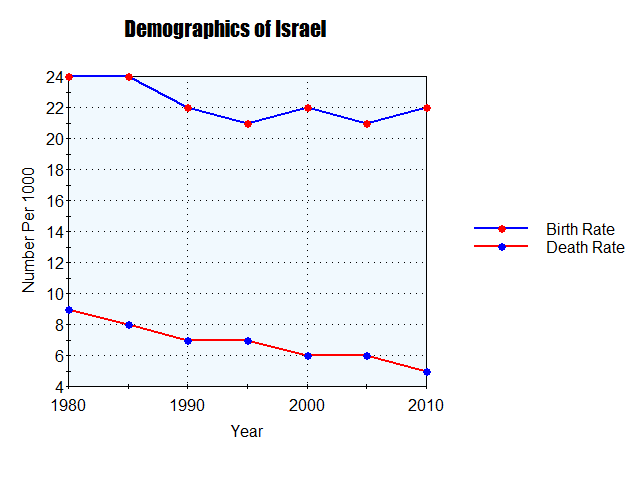
\includegraphics[width=8cm, height=6cm]{birthrate.png}
\\
Some quick GDP Facts [6]:
\begin{itemize}
	\item GDP growth rate = 0.70\%
	\item GDP annual growth rate = 2.9\%
	\item GDP growth annualized = 2.7\%
	\item GDP per capita = 33783.00 (USD)
	\item GDP per capita PPP = 32612.7 (USD)
	\item GDP constant prices = 309608.70 (ILS Million)
	\item Gross National Product = 310905.90 (ILS Million)
\end{itemize}

\begin{center}
GDP Per Capita [6]
\end{center}
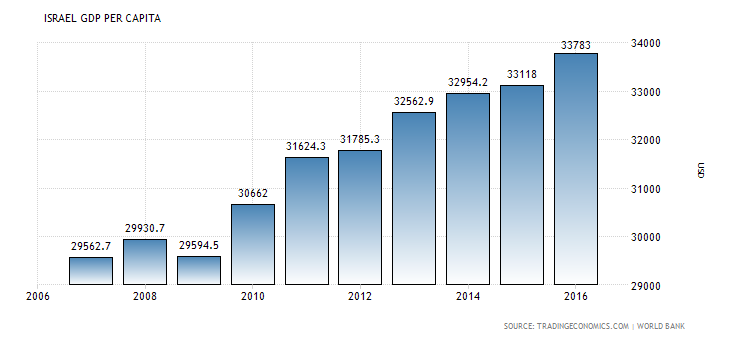
\includegraphics[width=10cm, height=6cm]{capita.png}
\\
\begin{center}
Population [6]
\end{center}
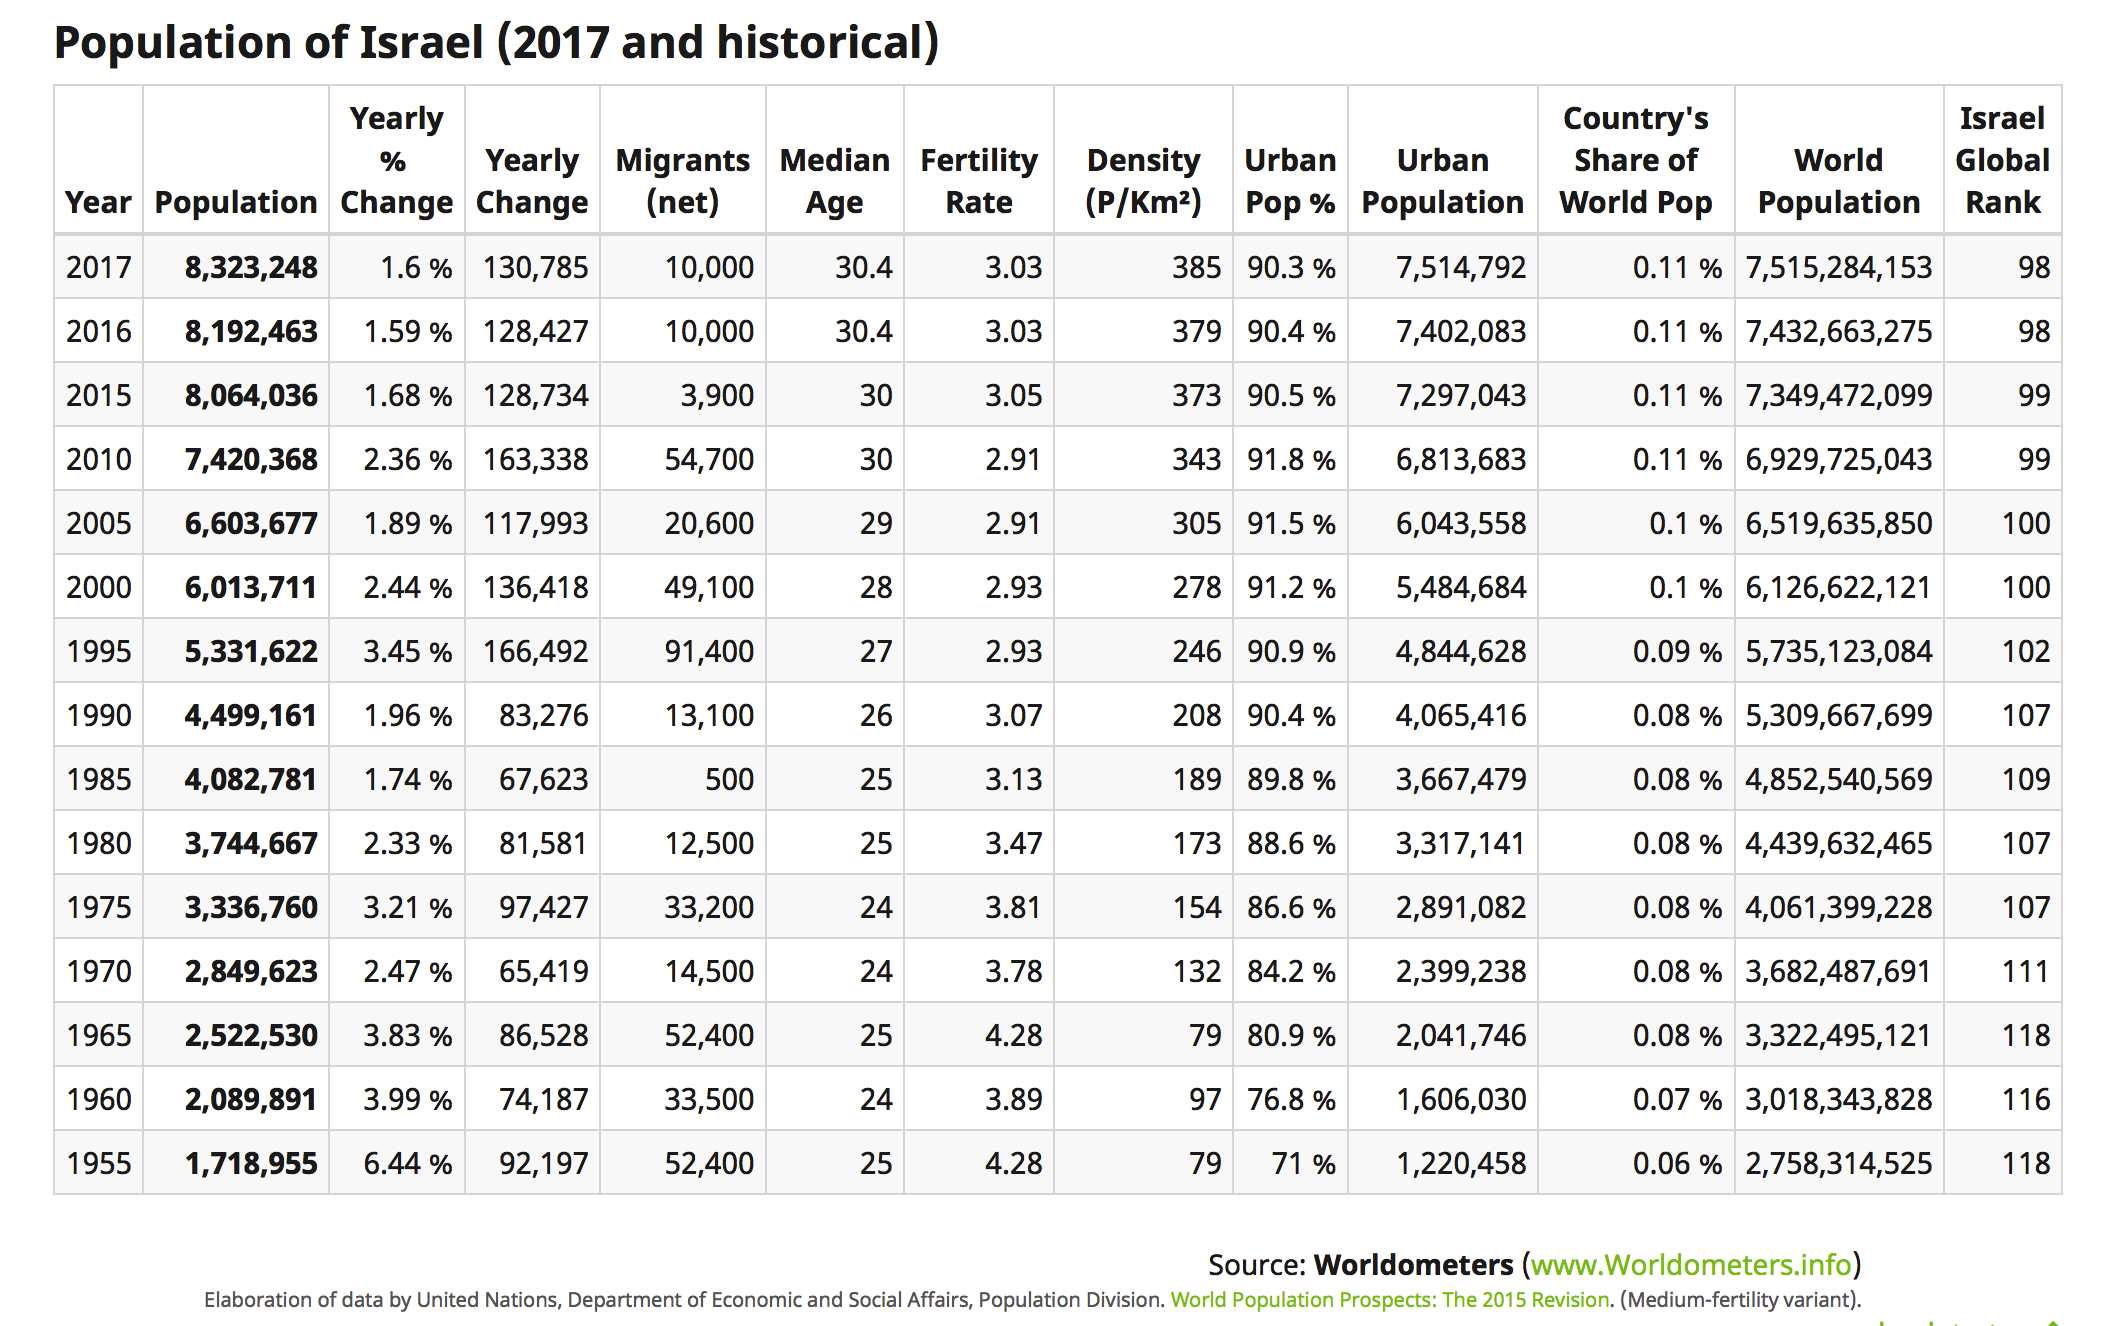
\includegraphics[width=16cm, height=10cm]{popula.png}
\\
\begin{center}
Sex Ratio [6]
\end{center}
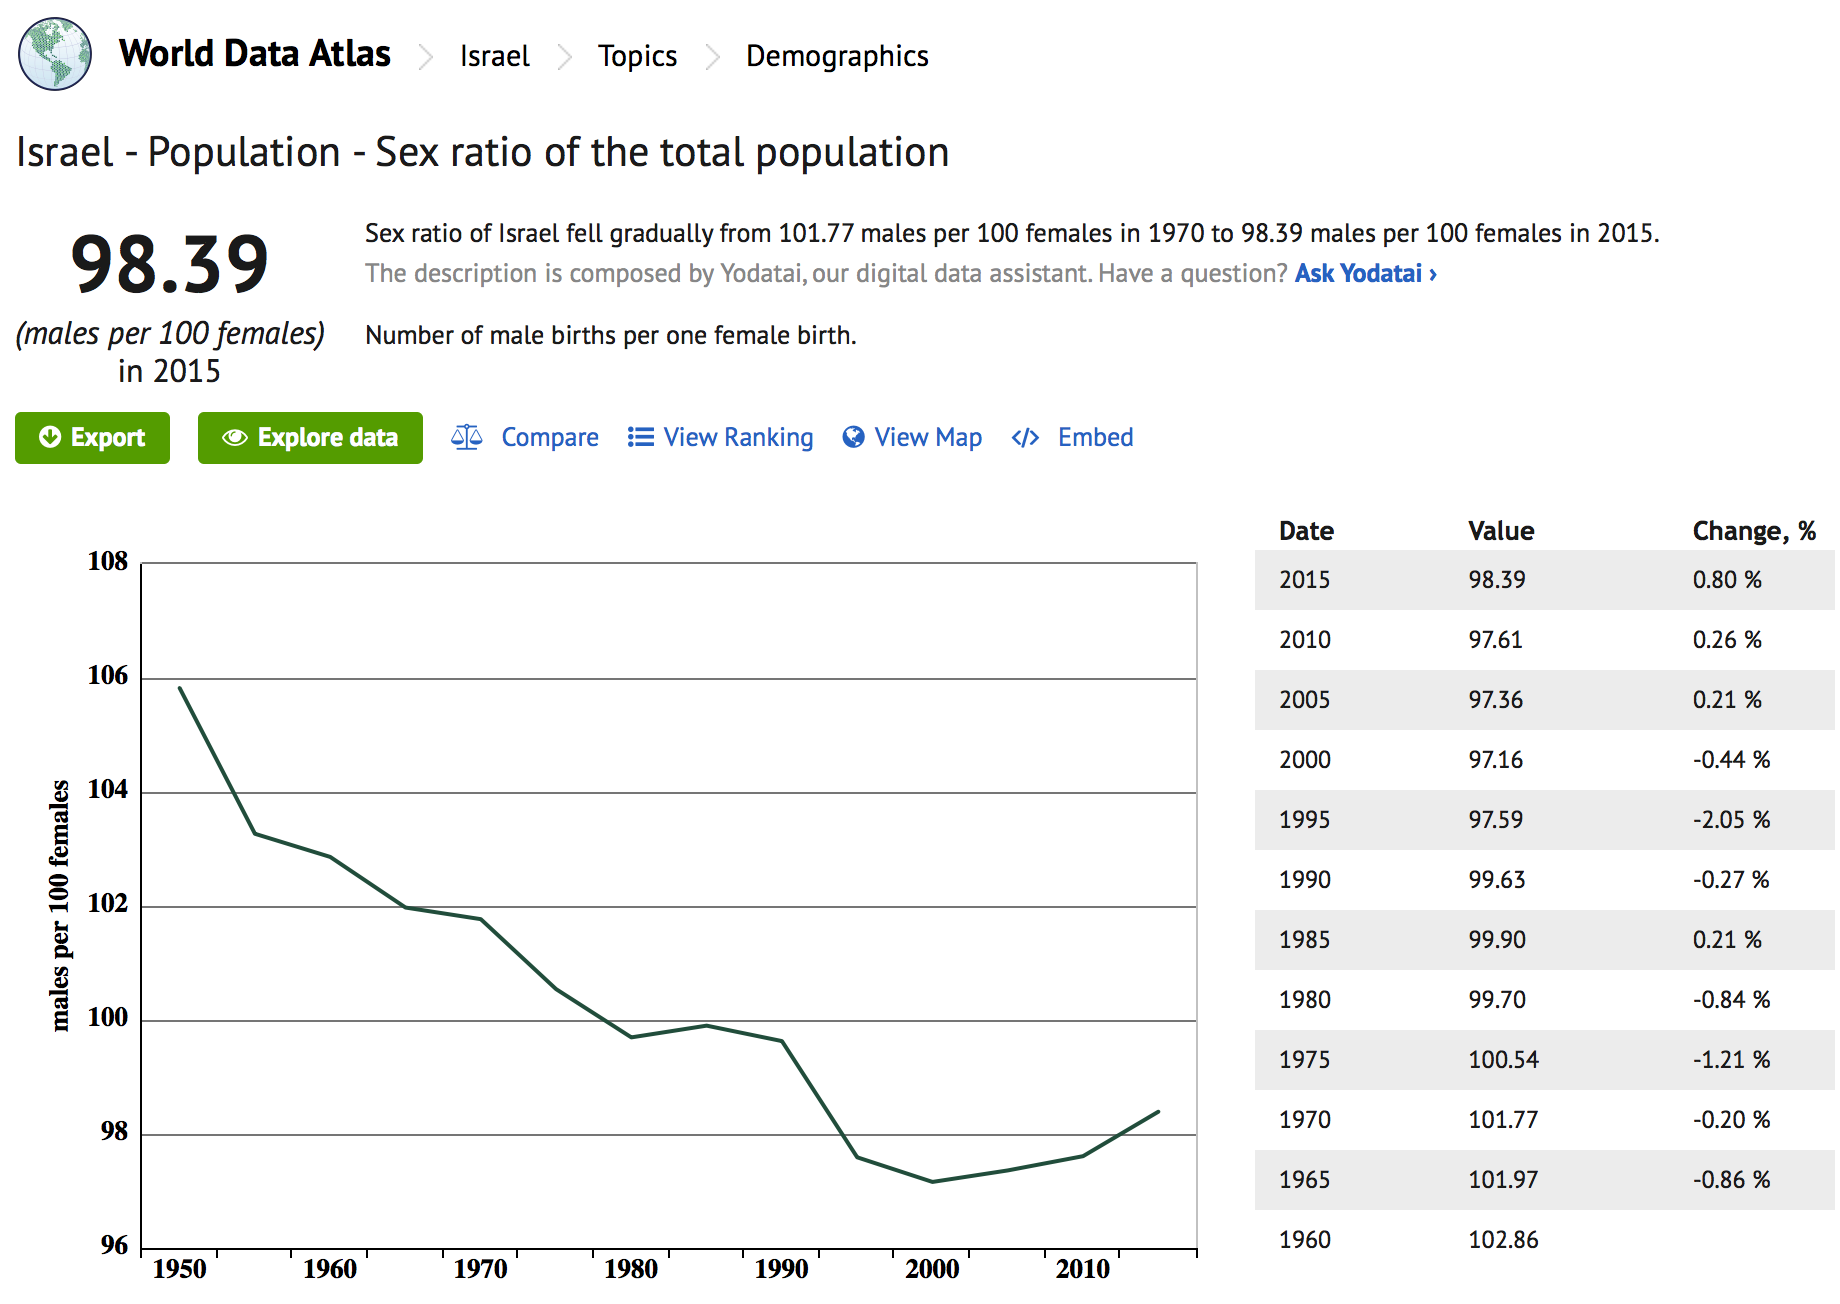
\includegraphics[width=14cm, height=10cm]{sexratio.png}
\\
\begin{center}
Exports to Other Countries [6]
\end{center}
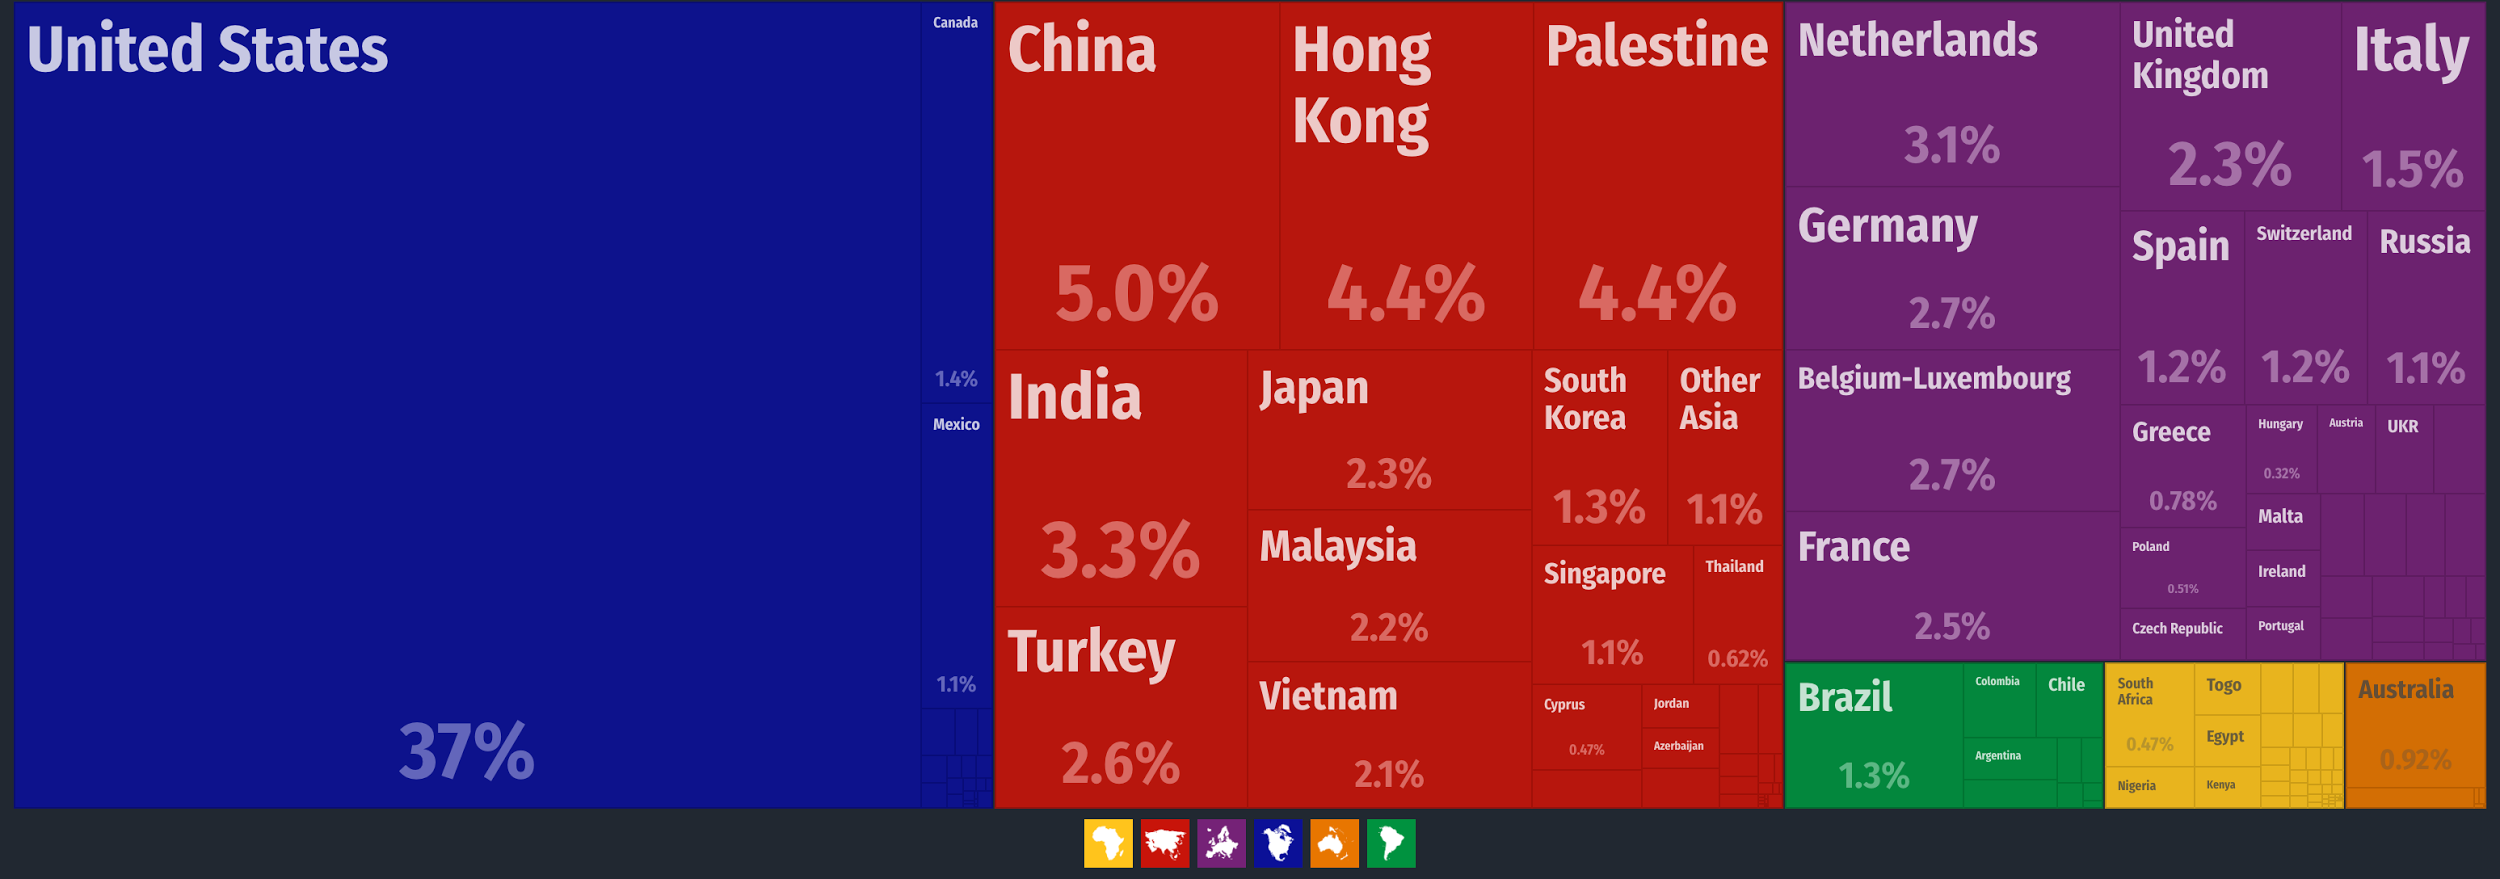
\includegraphics[width=6in, height=6cm]{exports.png}
\\
\begin{center}
Export Goods [6]
\end{center}
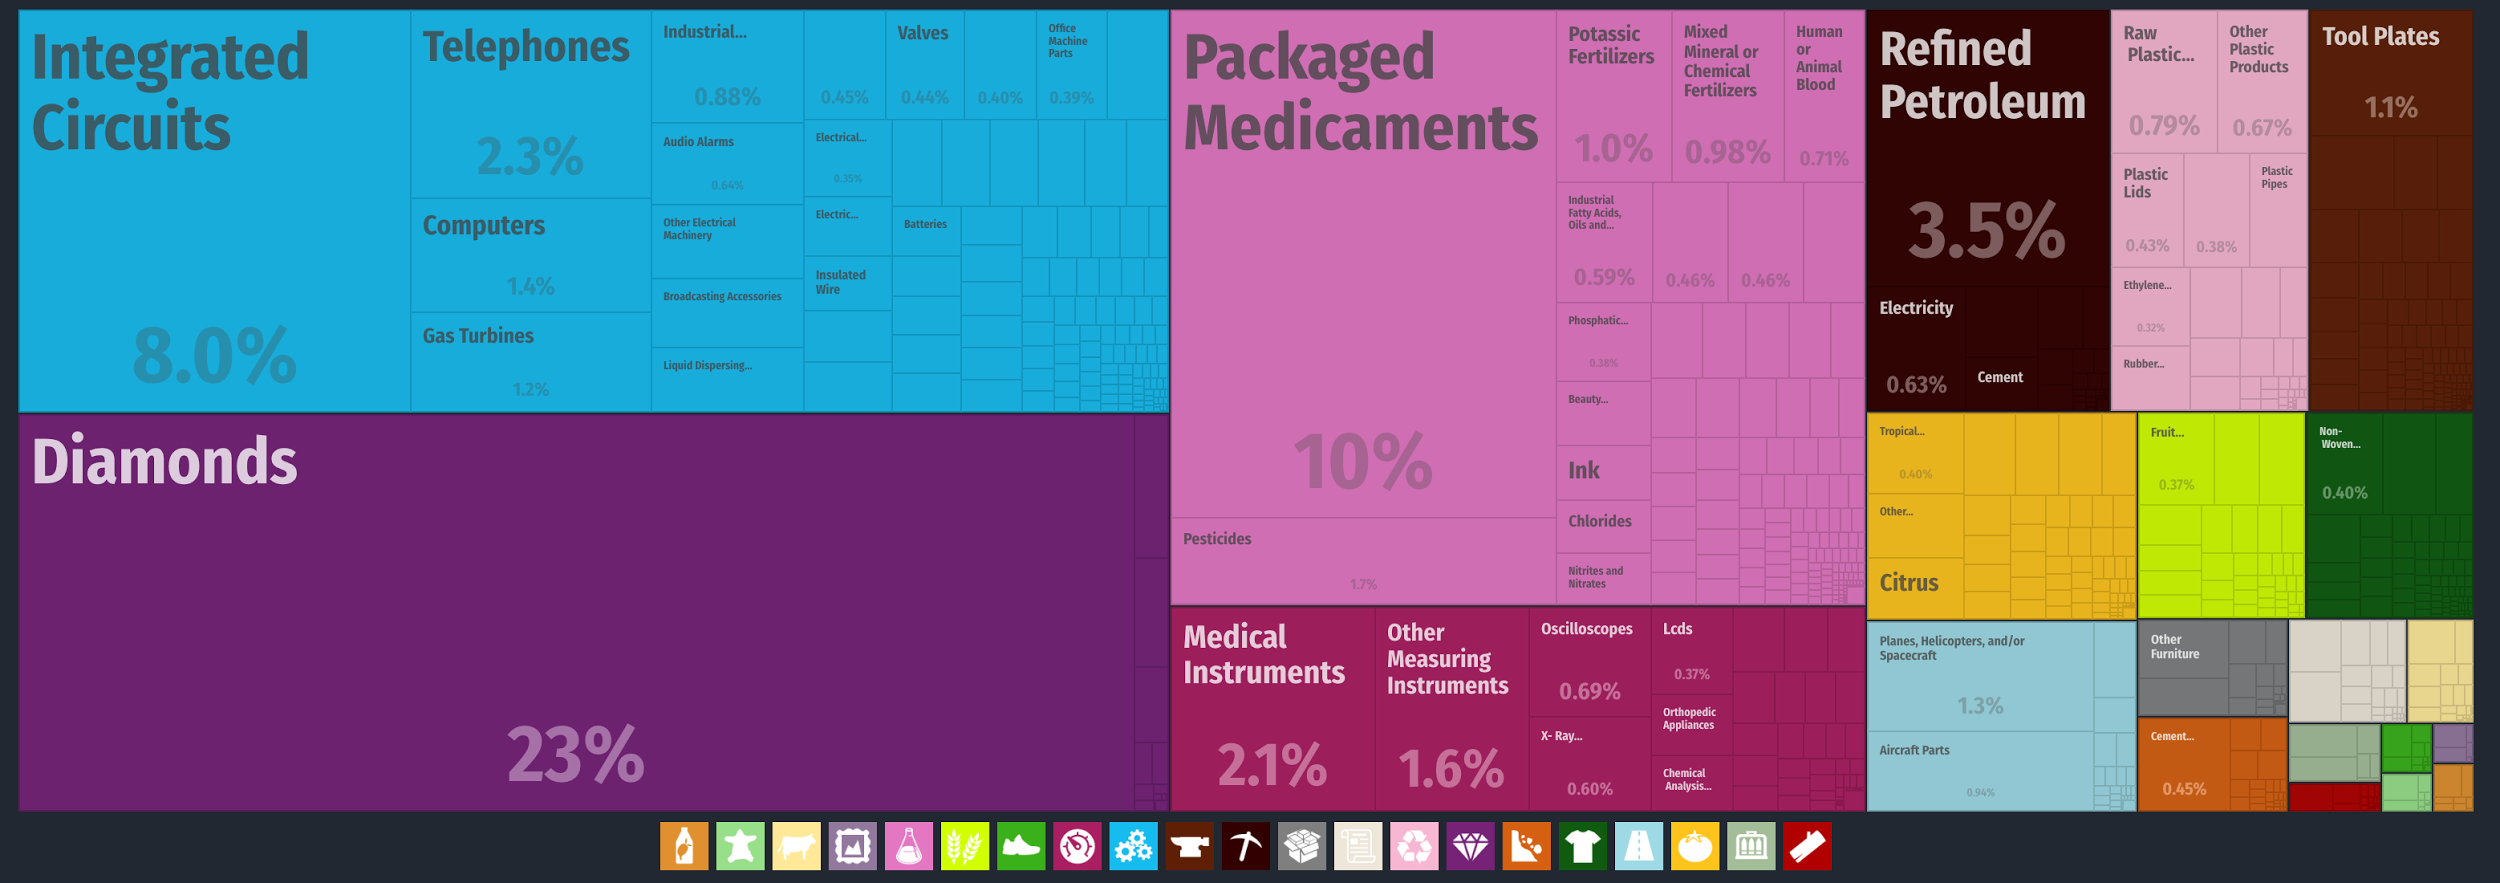
\includegraphics[width=6in, height=6cm]{exports1.png}
\\
\begin{center}
Import Goods [6]
\end{center}
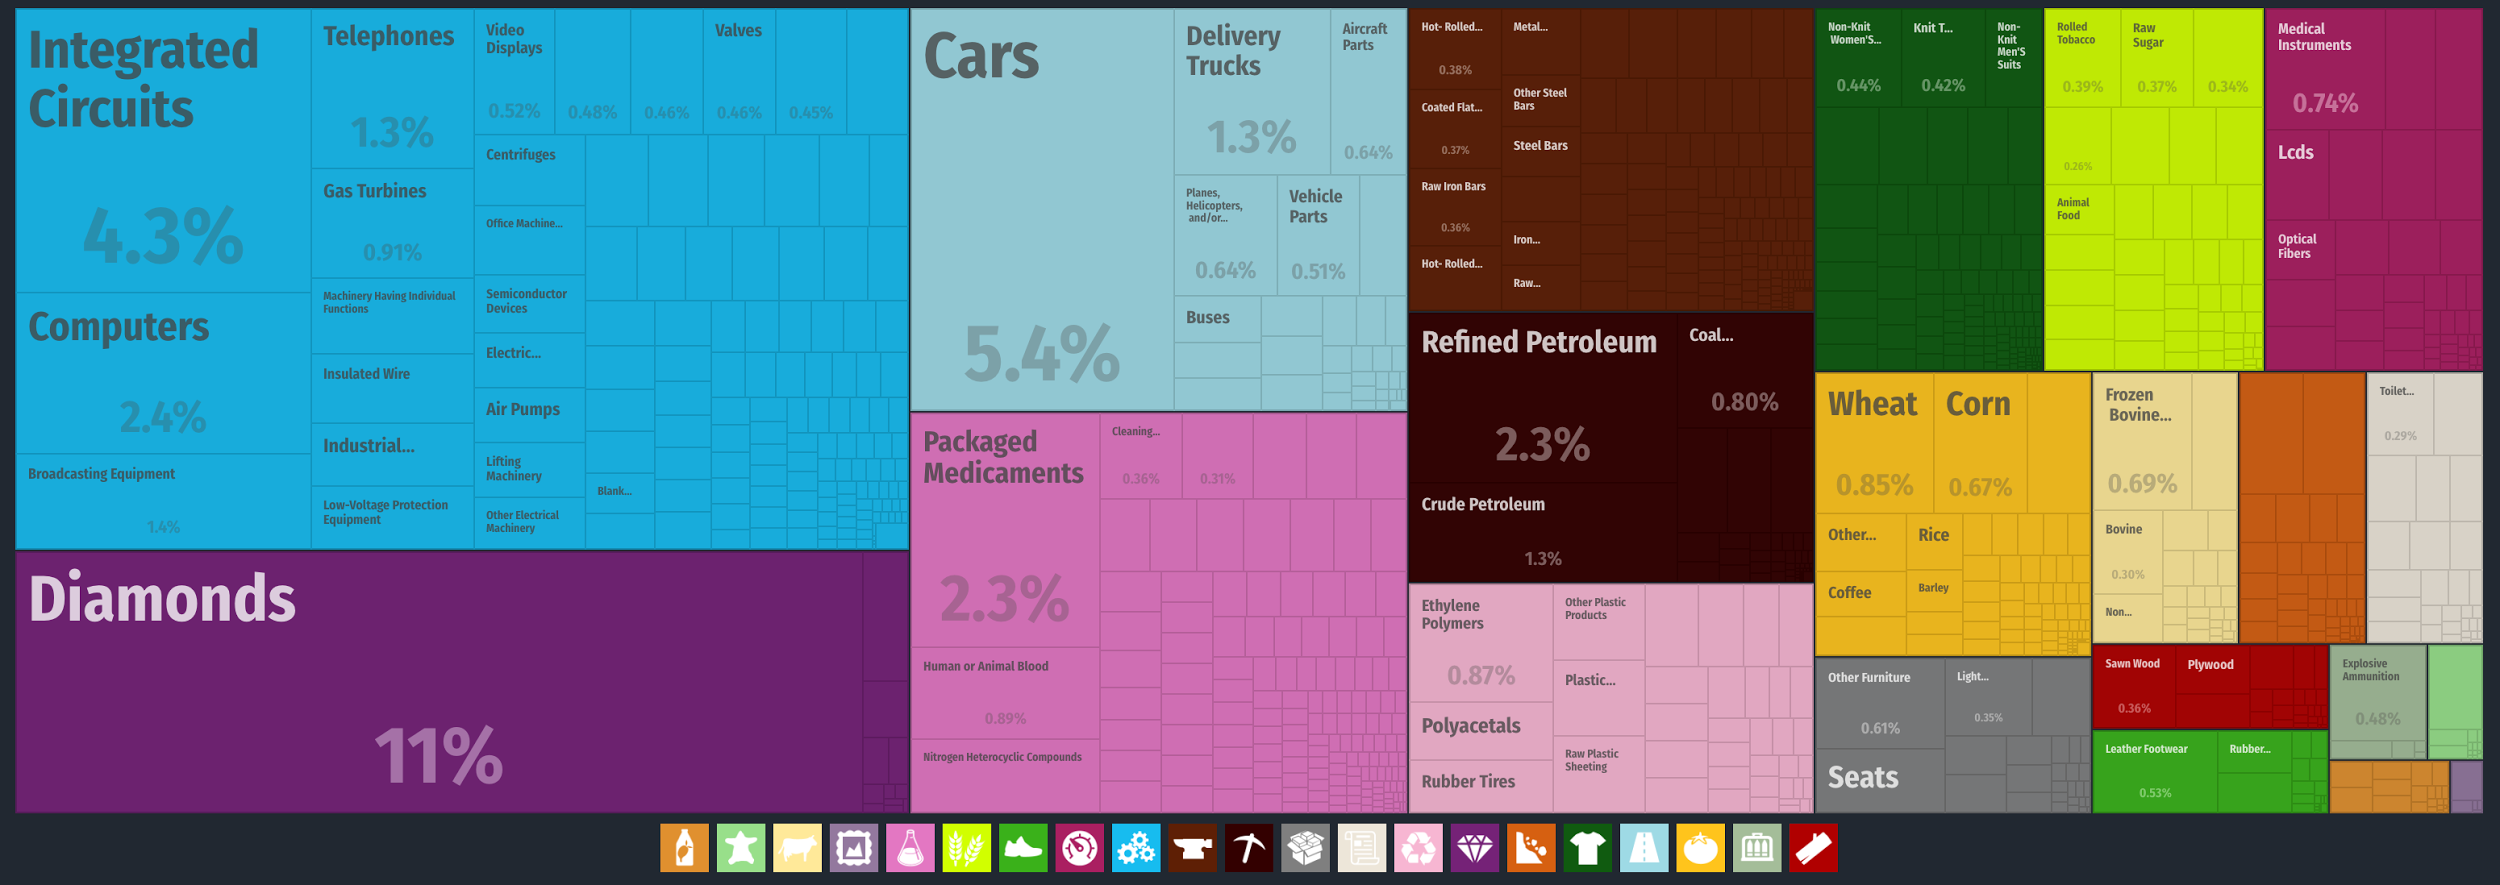
\includegraphics[width=6in, height=6cm]{imports.png}
\\
\newpage
\begin{center}
Imports form Other Countries [6]
\end{center}
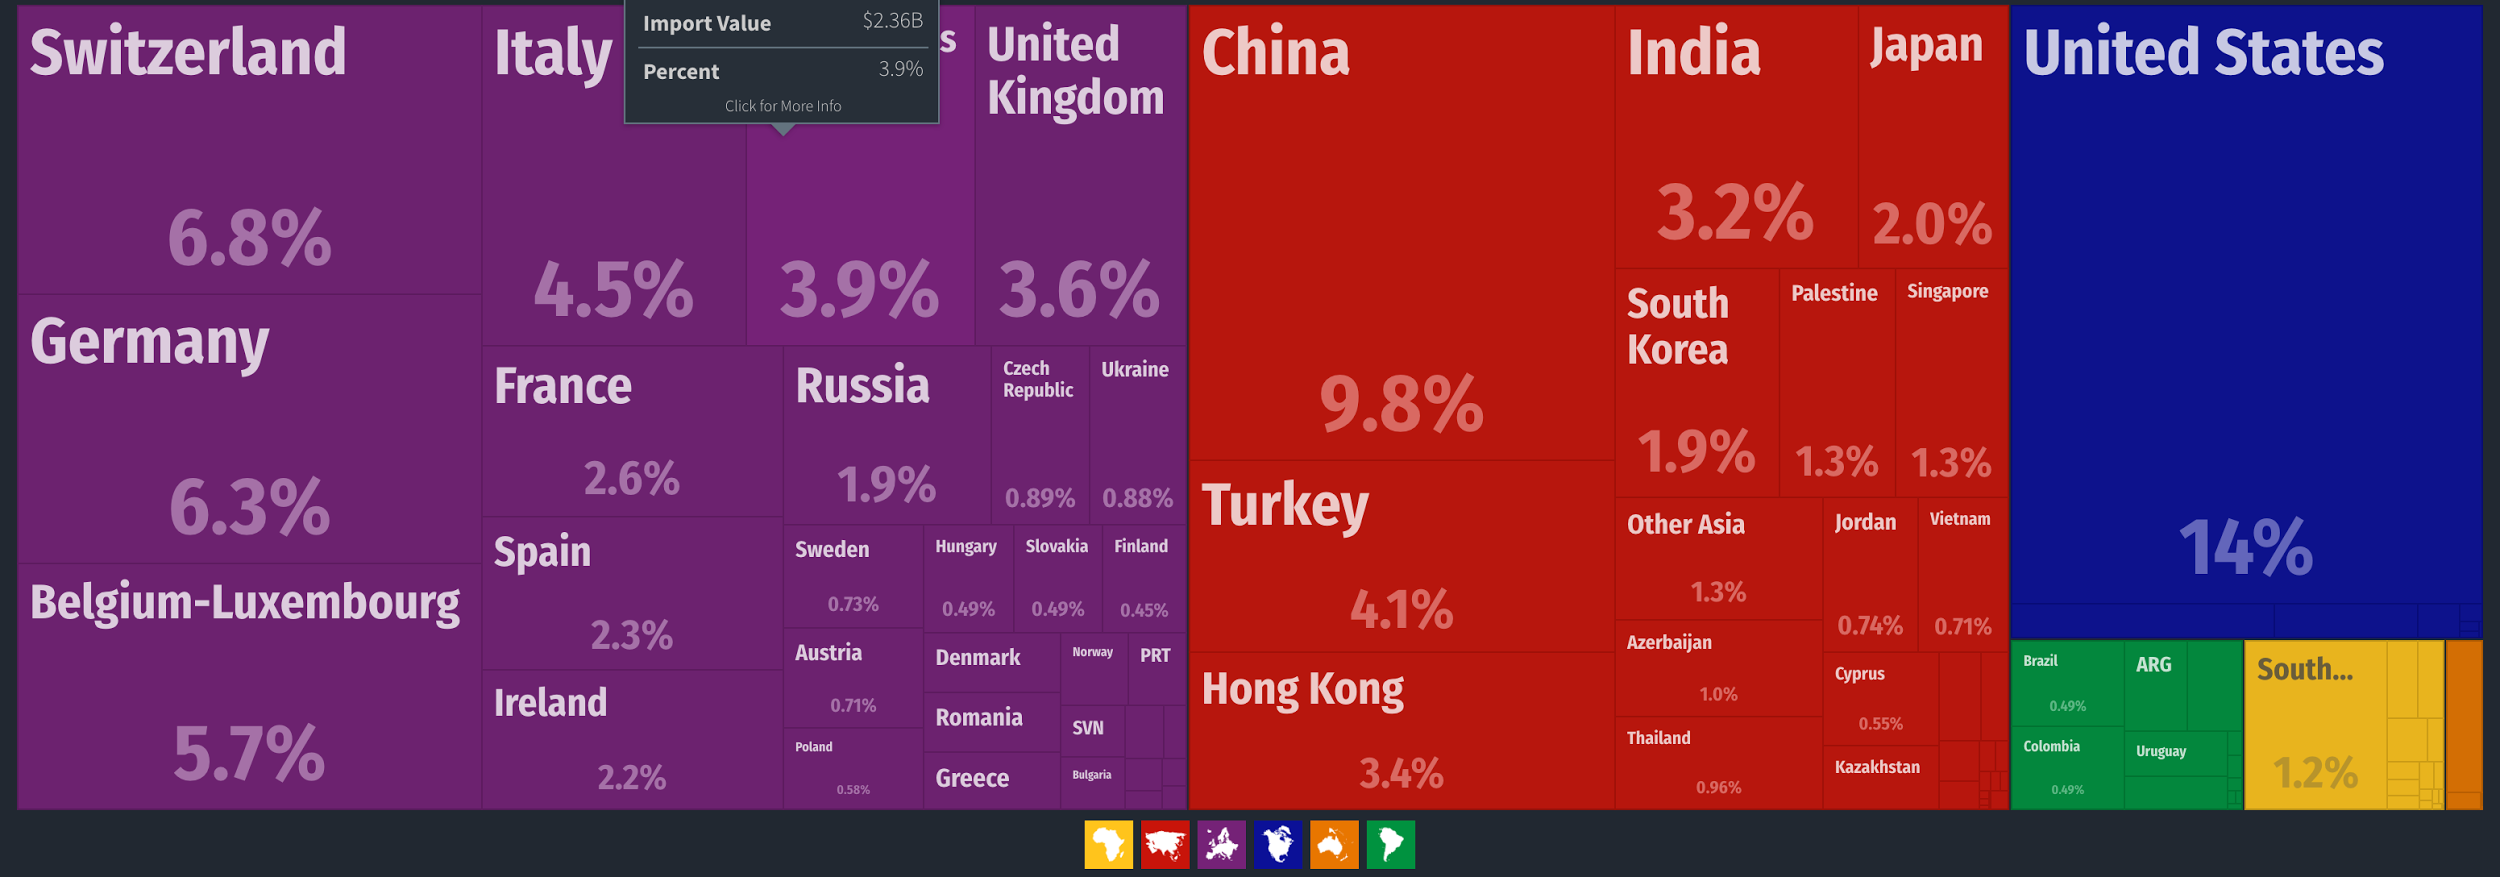
\includegraphics[width=6in, height=6cm]{imports1.png}

\subsection{Political Summary}
Despite an extremely diverse society marked with cultural and political differences, Israel remains one of the more stable countries in the Middle East. Owing to the polarity between secular and ultra-Orthodox Jews, Jews of Middle Eastern and European descent, and the split between the Jewish majority and the Arab Palestinian minority, Israel suffers with a very fragile political structure. Israel’s fragmented political scene invariably produces year on year, large coalition governments but there is a strong commitment to the rules of the parliamentary democracy [9].
\\
\\
Politics in Israel is never rests and important shifts in the country's political direction over the past two decades have had considerable effects on the Socio-Political situation. Israel has moved away from the economic model built by the early founders of the state, toward more liberal policies with a greater emphasis for the private sector. The economy prospered as a result, but the economic gap between highest and lowest strata widened resulting in harsh living conditions for the poorer section of the society [9].
\\
\\
The immediate future generation of Israelis find it increasingly difficult to secure stable employment and affordable housing among other issues such as the rise of prices of basic goods. In 2011, a wave of mass protest erupted, where hundreds of thousands of Israelis of different backgrounds demanded more social justice and jobs. There is a strong sense of uncertainty in the hearts of the younger population over the future and a lot of resentment against the political class as a whole [9].
\\
\\
Prime Minister Benjamin Netanyahu came on top of the parliamentary elections held on January 22. Netanyahu faces tough times in backing controversial budget cuts that were extremely unpopular with Israelis who were still struggling to keep up with rising prices.
\\
\\
In early 2011, a series of anti-government groups in Arab countries known as 'Arab Spring' threatened to disrupt the relatively stable geopolitical balance Israel had enjoyed in recent years. Interestingly, Egypt and Jordan are the only Arab countries that recognize the State of Israel, and Israel’s long-time ally in Egypt, former president Hosni Mubarak, had already been swept away and replaced with an Islamist government [9]. 
\\
\\
The relations with the rest of the Arab world are unstable to say the least and even hostile. Israel has few ally countries in the region. The once close strategic relationship with Turkey has disintegrated, Israeli policy makers fret over Iran’s nuclear program and its links to Islamist militants in Lebanon and Gaza, presence of Al Qaeda-linked groups among the rebels fighting the government troops in Syria is the latest item on the security agenda. The future of the peace process exhibits no potential [9].

\subsection{Contemporary Political and Economic Issues}
In November 2015, the Europe Union collectively decided to impose a label on goods that originated from the so called 'Israeli-occupied territories'. The Economy Minister of Israel estimated at that time the impact of this decision would be about \$50 million a year. Although this may be eclipsed by the fact that every year Israel exports \$30 billion worth of goods and services to EU alone. The EU also requires any private Israeli entity that wants to receive any sort of funding form EU to show that it has no links to the West Bank, East Jerusalem, or the Golan Heights region. The EU deems territories such as Jewish communities in the West Bank, East Jerusalem and the Golan Heights as 'occupied territories'). EU aims to limit the finance for new settlements in these areas [10].
\\
\\
One strong parameter to gauge Europe's negative political attitude towards Israel is its voting record in the United Nations (UN). Europe's voting at the UN is influenced by the EU and shows a long-standing anti-Israeli bias. Every year the UN General Assembly passes between 18 and 22 anti-Israeli resolutions and generally speaking, the Europeans support these resolutions [10]. Another example of EU political bias is seen in the frequent condemnations of Israel from Brussels. In recent years the United States of America, Israel's strongest ally has sunk to an all time low. This can be attributed to Israel’s pursuit of her settlement policies on the West Bank and her building policies in Jerusalem.
\\
\\
As of 2013, the UN Security Council had adopted 77 resolutions critical of Israel and only 1 against the Palestinians [10]. The United Nations makes no mistake regarding its position in this situation. As of 2012, the UN had passed 79 resolutions critical of Israel, and 40\% of UN Human Rights Council Resolutions have been against Israel. EU bias became clear in 2014 when the parliaments of Sweden, Britain, France, Spain, Ireland, Portugal and Luxembourg voted in support of recognizing, in principle, a Palestinian state within the 1967 borders [10]. For her part, Israel continues to ignore such resolutions.
\\
\\
Israel’s relationship with Islamic countries, notably Iran, is non-existent. Iran maintains that there can be no two-state solution and that there can be only one state and that would be called Palestine under Muslim rule. The international political situation is rapidly aligning itself to Bible prophecy which states that at the end of this age all nations will be aligned against Israel. Israel suffers from unwarranted international prejudice or bias against her. This result in widespread misunderstanding and ignorance of the true nature and purpose of Israel. This bias comes from the general public, the media, political organizations (as in the UN and EU), and even the church (as in the World Council of Churches, WCC). Collectively, they all aim to change Israeli government policy that specifies ownership and use of land e.g. land boundaries, and with respect to Israel’s claim on Jerusalem. At its extreme, bias aims to bring down the country and destroy it.
\\
\\
Legal misinformation again from the media, leads to the frequent but inaccurate claim that 'Israel occupies Palestinian land'; legally it does not. Sadly, the World Council of Churches (WCC) tends to follow this misinformation, link, and the institutionalized churches e.g. the Anglican Church lean to the view that the church has replaced Old Testament Israel (Replacement Theology) [11].

\section{Societal and Technological Landscape}
Israel’s answer to Silicon Valley is Silicon Wadi, an area around Tel Aviv on the country's coastal plain with a heavy concentration of high-tech industries that rivals the San Francisco Bay Area’s cluster of innovative firms. Israel continues to produce an impressive number of highly successful tech companies for a country with a population of just 9 million people. It is sometimes referred to as "Startup Nation" thanks to the sheer number of entrepreneurs building businesses there, particularly in cities like Tel Aviv. Multinational tech companies like Google, Apple, Facebook, and Microsoft all have research centres in Israel but some of the local companies are arguably more interesting, with many of them specialising in drones, cybersecurity, and autonomous driving technology [13].

\subsection{Today's Society}
Nearly 70 years after the establishment of the modern State of Israel, the residing Jewish population remains united behind the idea that Israel is a homeland for the Jewish people. But alongside unity, deep divisions in Israeli society – not only between Israeli Jews and the country’s Arab minority, but also among the religious subgroups that make up Israeli Jewry can be found [12].
\\
\\
Jews in Israel broadly identify themselves with one of four categories: Haredi (commonly translated as 'ultra-Orthodox'), Dati (“religious”), Masorti (“traditional”) or Hiloni (“secular”). Although they live in the same small country and share many traditions, highly religious and secular Jews live largely separate social worlds, with relatively few close friends and little intermarriage outside their own groups. In fact, secular Jews in Israel are more uncomfortable with the thought that a child of theirs might someday marry an ultra-Orthodox Jew than they are with the prospect of their child marrying a Christian [12].
\\
\\
Moreover, these divisions are reflected in contrasting positions of these groups on many public policy questions, including marriage, divorce, religious conversion, military conscription, gender segregation and public transportation. It is common to witness Haredi and Dati Jews (both generally considered Orthodox) express the view that Israel’s government should promote religious beliefs and values, while secular Jews strongly favour separation of religion from government policy [12].
\\
\\
Most Jews across the religious spectrum agree that Israel can be both a democracy and a Jewish state. But confusion and uncertainty seeps, especially when situations where democratic decision-making collides with Jewish law (halakha). The majority of secular Jews say democratic principles should take precedence over religious law, while a similarly large share of ultra-Orthodox Jews say religious law should take priority [12].
\\
\\
"Even more fundamentally, these groups disagree on what Jewish identity is mainly about: Most of the ultra-Orthodox say “being Jewish” is mainly a matter of religion, while secular Jews tend to say it is mainly a matter of ancestry and/or culture." - Source [12]
\\
\\
To be sure, Jewish identity in Israel is complex, consisting of diverse thoughts in religion, ethnicity, nationality and family. Most secular Jews in Israel say they see themselves as Israeli first and Jewish second, while most Orthodox Jews (Haredim and Datiim) say they see themselves as Jewish first and then Israeli.

\subsection{Technology }
One of the more established players in both Silicon Valley and its Middle Eastern rival, Israel's own 'Silicon Wadi', is Intel Corporation, which set up a research and production operation in Israel in 1972. Since then, Intel Israel has grown to the point where it has become Israel’s largest private employer, with more than 10,200 workers on its payroll as of last year. According to Maxine Fassberg, executive in residence and vice president of Intel Capital, the company exported \$3.35 billion of chips and other products from Israel last year, accounting for 1\% to 2\% of the country’s GDP [13].
\\
\\
Today, Israel allocates a higher percentage of its G.D.P. to Research and Development (R\&D) than any other country, and roughly 30 percent of Israeli R\&D goes toward military technologies. Israel also invests in its human resources, with numerous specialized educational programs that are offered at various institutions designed to bring top talent. Israel’s small size, combined with its tradition of universal military service helps by ensuring that there's rarely more than one degree of separation between military officials, scientists and entrepreneurs; as a result, military needs and challenges are quickly and easily communicated to policy makers, academics and financiers [17].
\\
\\
Israel attracts about 15\% of the world’s venture-capital investment in cyber-security. Israels booming 'Statup-Nation' economy us the most dynamic innovation ecosystem outside of America. Direct flights now connect San Francisco to Tel Aviv. Other high-tech areas look promising, too, among them agricultural and water technology (building on Israel’s expertise in desert farming), digital health services and financial technology. Intrestingly, during the 1980s, Israel was on the brink of financial collapse. Its near-defeat in the Yom Kippur war had caused it to push defence spending to an extraordinary 30\% of GDP in 1975. By 1984 public debt had reached nearly 300\% of GDP and hyperinflation peaked at 450\% a year [14].
\\
\\
Many bilateral ties with other countries tightly evolve around the technological development of and form Israel. On the second day of Prime Minister Benjamin Netanyahu’s visit to China, Israel and China took further steps to strengthen economic and scientific relations. Israeli and Chinese ministers and top officials signed 10 bilateral agreements in health, science, education, environmental protection and other areas. Addressing dozens of Israeli and Chinese government officials, industry leaders, university presidents and private businesspeople, Netanyahu called on Beijing to accelerate the pace of negotiations over an Israel-China free trade agreement, which started exactly one year ago. Netanyahu said that in today’s world everything is becoming technologized and that therefore all countries need to innovate. He hailed Israel’s startup scene, highlighting Intel’s recent acquisition for \$15 billion of Jerusalem-based autonomous driving company Mobileye, adding that Israel is home to 500 additional companies “that do the same thing. A few years ago we had nothing.” [15].
\\
\\
Despite hosting a rich startup ecosystem, Israel's relatively smaller population pose as obstacles to entrepreneurs seeking to build big companies. As a result, Israeli entrepreneurs need to begin immediately thinking outside of Israel since their primary market is often the U.S. The common approach is to incubate the business locally in Israel with a small development team, prove early product/market fit, and then build a sales and marketing organization abroad, usually in the U.S. In the old model of Israeli startups, many Israeli executive teams would hire a vice president of sales in the U.S. to assist with the local go-to-market approach [16].
\\
\\
Over the recent years, Israeli founders are themselves moving to the U.S. to build satellite offices and personally oversee recruitment and management of American executives. However, it has become evident lately that waiting to move to the U.S. right before the late-stage go-to-market phase may be too late. All of the risks intrinsic to launching a startup are overshadowed by the geographic distance between Israel and the U.S. hiring talent. Furthermore, gathering customer feedback challenges the organization when teams are so physically far apart, and this separation can make it harder to build culture, establish partnerships, and raise capital [16].
\\
\\
Over the past decade, the economy has grown at about 4\% a year. The unemployment rate is 4.3\%, a record low. The labour-force participation rate has risen. A country with few natural resources plans to export gas to Europe from its offshore fields, and is selling water to Jordan as major technological advancements in water desalination gathers pace. Public debt has come down to 62\% of GDP, the current account is in surplus and foreign-currency reserves are high. All significant transactions were once reckoned in dollars; the worry now is the strength of the shekel, which has appreciated by 13\% against a basket of currencies in two years. The central bank periodically intervenes in foreign-exchange markets to hammer it down. Israel has not had a recession since the height of the second intifada [14].
\\
\\
However, its not all good news. With all the recent developments, the income gap between the rich and the poor continues to increase. With GDP per person at \$35,700 a year in 2015, Israel’s standard of living is nearly the same as that of France. Meanwhile, in West Bank, the figure stands at \$3,700, placing it in the ballpark of Egypt and for Gaza it is about \$1,700, similar to Congo-Brazzaville’s [16].

\section{Miscellaneous}

\subsection{Water}
The intense scarcity of water in Israel has led to the increase in their efforts to maximize their use of available supply and to seek new resources. The National Water Carrier, which brings water from the north and the center of the semi-arid south in 1960’s joined Israel's fresh water resources in an integrated grid. Israel currently has many ongoing projects for recycling and finding new sources of water some of them are cloud seeding, recycling of sewage and desalination of seawater [18]. 

\subsection{Education and Science}
In Israel attendance is a mandatory from ages five, and free through age 18. Preschool programs are attended by almost all 3-4-year-old. Israel has world class universities covering a wide range of subjects such as science and humanities, and serving as research Institutes of worldwide repute. The features like high level scientific research and development and the application of R\&D compensate for the country's lack of natural resources.

\subsection{Health}
In January, 1995, a law was passed called the National Health Insurance Law, which provides a standardized basket of medical services, for all residents of Israel including hospitalization. All medical services continue to be supplied by the country's four health care organizations. For women, the life expectancy rate is being 83.4 years and for men it is 79.7. Infant mortality rate stands at 4.0 per 1000 live births [18].
 
\subsection{Social Welfare}
The legislation produces the country with a large range of national and community services, including care of the elderly, programs for children and youth and adoption agencies. As well as prevention and treatment of alcoholism and drug abuse. The National Insurance Institute gives Israeli citizens with a large range of national and community services, including care of the elderly, unemployment insurances, old age pensions, and more [18]. 
 
\subsection{Agriculture}
The successes of Israel are the result of a long struggle against harsh and adverse conditions and making use of very less water and arid land. Agriculture represents some 2.4\% of imports of GNP and 2\% of exports, Israel produces a 93\% of its own food products, supplemented by imports of various food products like oil seeds, grain, meat and cash crops [18].

\subsection{Water Related Issues}
Israel is the numero uno in recycling of water in the world and over 80\% of the water is recycled for agriculture. This is a major achievement and no other nation is even close to this system. Adding to these hundreds of reservoirs have been built with the help of countries top notch engineering companies. Some solutions such as solar power stations and covering of water surface are to be considered and this solution also increases the utility of land and further may be very useful in the future when electricity produced from exhaustible resources become way too costly [20]. 
\\
\\
A decade ago, Israeli water management was on the edge of a catastrophe the results were several years of drought, diminishing aquifers, and water reservoirs in addition to increasing water demand which has a deadly combination. The lower price of desalination of sea water became a real success for them and this advancement of technology was a milestone in the world of recycling. Constructing of huge desalination projects were financially feasible. The Israeli government supported this by investing significant sums in developing such infrastructure on the Mediterranean. In 2015, 40\% of the drinking quality water is produced through desalination process. A slip slide of desalination it requires huge energy requirements and thus requires cheap energy resources and thus solar energy was used in developing solar desalination [20].
\\
\\
The quality of drinking water in Israel is unsatisfactory and is expected to decline due to the taste of chlorine. This is the conclusion of the ministry of health is obliged to advise residents in certain areas to boil their drinking water and the quick increase in the sale of packaged drinking water is considered a high rank luxury a few years ago. Moreover, the quality of water in Israel is a major motivation for them to be concerned about it and having efforts to save water, particularly in agriculture. Today Israel is the leader in utilization of 'grey water', that is water recycled from sanitary sewage [19].
\newpage

\begin{thebibliography}{1}
\bibitem{fo} Israel - World FactBook {\em https://www.cia.gov/library/publications/the-world-factbook/geos/print\_is.html} : Central Intelligence Agency.

\bibitem{fo} Israel Facts {\em https://www.buzzfeed.com/rethinkisrael/facts-about-israel-that-will-surprise-you?utm\_term\=.mk02QqY6M7\#.ij4YPD9eAj} : BuzzFeed.

\bibitem{fo} History of Israel {\em http://embassies.gov.il/pretoria/AboutIsrael/history/} : Embassy of Israel.

\bibitem{fo} About Israel {\em http://embassies.gov.il/UnGeneva/AboutIsrael/Pages/AboutIsraelgeneralinfo.aspx} : Embassy of Israel.

\bibitem{fo} Geography and Climate In Israel {\em http://mfa.gov.il/MFA/AboutIsrael/Land} : Ministry of Foreign Affairs, Israel.

\bibitem{fo} Israel {\em https://data.oecd.org/israel.htm} : OECD Data.

\bibitem{fo} Sectors of Israel's Economy {\em http://www.mfa.gov.il/mfa/aboutisrael/economy/pages/economy-\%20sectors\%20of\%20the\%20economy.aspx} : Ministry of Foreign Affairs, Israel.

\bibitem{fo} Tourism - Israel {\em https://www.gov.il/en/Departments/ministry\_of\_tourism} : Ministry of Tourism, Israel.

\bibitem{fo} Current situation In Israel {\em https://www.thoughtco.com/current-situation-in-israel-2353137} : Thought Co.

\bibitem{fo} World bais against Israel {\em http://www.factsaboutisrael.uk/world-bias-against-israel/} : Facts About Israel.

\bibitem{fo} Israeli - Palestinian Conflict {\em http://www.factsaboutisrael.uk/israeli-palestinian-conflict/} : Facts About Israel.

\bibitem{fo} Israels divided Society {\em http://www.pewforum.org/2016/03/08/israels-religiously-divided-society/} : PewForum.

\bibitem{fo} Israels Tech Startups are giving Silicon Valley a run for its money {\em http://nypost.com/2017/05/28/israels-tech-startups-are-giving-silicon-valley-a-run-for-its-money/} : New York Post.

\bibitem{fo} Israel’s economy is a study in contrasts {\em https://www.economist.com/news/special-report/21722037-dazzling-high-tech-firms-divert-attention-serious-productivity-problem-israels} : The Economist.

\bibitem{fo} Netanyahu looks to marry Israels technology with China {\em https://www.timesofisrael.com/in-beijing-netanyahu-looks-to-marry-israels-technology-with-chinas-capacity/} : Times Of Israel.

\bibitem{fo} How Israeli startups can scale {\em https://hbr.org/2015/09/how-israeli-startups-can-scale} : Harvard Business Review.

\bibitem{fo} Israel’s Military-Entrepreneurial Complex Owns Big Data {\em https://www.technologyreview.com/s/516511/israels-military-entrepreneurial-complex-owns-big-data/} : MIT Technology Review.

\bibitem{fo} About Israel {\em http://embassies.gov.il/UnGeneva/AboutIsrael/Pages/AboutIsraelgeneralinfo.aspx} : Embassy of Israel.

\bibitem{fo} Environmental Issues In Israel {\em http://www.jewishvirtuallibrary.org/environmental-issues-in-israel} : Jewish Virtual Library.

\bibitem{fo} Encountering Environmental Challenges in Israel {\em http://www.jpost.com/Blogs/From-Green-Finland-to-Yellow-Arava/Encountering-Environmental-Challenges-in-Israel-in-the-beginning-of-a-New-Year-432787} : JPosts.

\end{thebibliography}

\end{document}